%!TeX root=../main.tex
\textbf{Classification}\:
%
Promising results on reinforcement learning tasks lead us to consider how widely a WANN approach can be applied. WANNs which encode relationships between inputs are well suited to RL tasks: low-dimensional inputs coupled with internal states and environmental interaction allow discovery of reactive and adaptive controllers. Classification, however, is a far less fuzzy and forgiving problem. A problem where, unlike RL, design of architectures has long been a focus. As a proof of concept, we investigate how WANNs perform on the MNIST dataset~\cite{lecun1998mnist}, an image classification task which has been a focus of human-led architecture search for decades~\cite{lecun1998gradient,chollet2015keras,sabour2017dynamic}.

% Shorten some of this, as these details are also in the supplementary (DH: moved to appendix for now)
%To fit into our existing approach MNIST classification is reframed as a reinforcement learning problem. Each sample in MNIST is downsampled to a 16x16 image, deskewed, and pixel intensity normalized between 0 and 1. WANNs are created with input for each of the 256 pixels and one output for each of the 10 digits. At each evaluation networks are fed 1000 samples randomly selected from the training set, and given reward based on the softmax cross entropy. Just as before networks are tested with a varied of shared weight values, maximizing performance over all weights while minimizing the number of connections.

% Better than a linear classifier
Even in this high-dimensional classification task WANNs perform remarkably well (Figure~\ref{fig:mnist}, Left). Restricted to a single weight value, WANNs are able to classify MNIST digits as well as a single layer neural network with thousands of weights trained by gradient descent. The architectures created still maintain the flexibility to allow weight training, allowing further improvements in accuracy.

%!TeX root=../main.tex

% TODO: Edit caption waaay down

\begin{figure}[!htb]        
\vskip -0.10in % useful knobs to optimize layout
    \centering        
    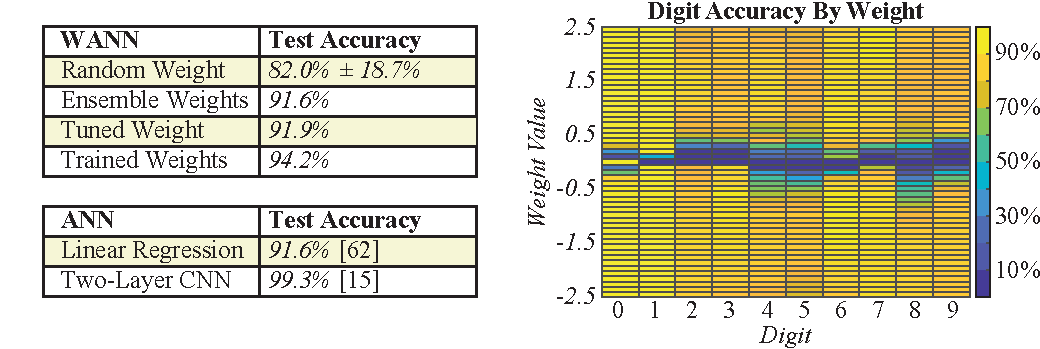
\includegraphics[width=1\textwidth]{img/mnist.pdf}   
\vskip -0.20in % useful knobs to optimize layout (going a bit overboard here, since caption is only on left side)
    \caption      
    {     
        \textit{Classification Accuracy on MNIST.
        }
        \newline
        \textit{Left:}
        WANNs instantiated with multiple weight values acting as an ensemble perform far better than when weights are sampled at random, and as well as a linear classifier with thousands of weights. 
        %
        %The accuracy of the best single weight value exceeds this. 
        \newline
        \textit{Right:} No single weight value has better accuracy on all digits. That WANNs can be instantiated as several \textit{different} networks has intriguing possibilities for the creation of ensembles.       
    }
    \label{fig:mnist}
\vskip -0.05in % useful knobs to optimize layout
\end{figure}

%

% Ensembles
It is straight forward to sweep over the range of weights to find the value which performs best on the training set, but the structure of WANNs offers another intriguing possibility.
%
At each weight value the prediction of a WANN is different.
%
On MNIST this can be seen in the varied accuracy on each digit (Figure~\ref{fig:mnist}, Right).
%
Each weight value of the network can be thought of as a distinct classifier, creating the possibility of using one WANN with multiple weight values as a self-contained~ensemble. % formatting weridness -> use ~ before ensemble

%

In the simplest ensemble approach, a collection of networks are created by instantiating a WANN with a range of weight values. 
%
Each of these networks is given a single vote, and the ensemble classifies samples according to the category which received the most votes.
%
This approach yields predictions far more accurate than randomly selected weight values, and only slightly worse than the best possible weight.
%
That the result of this naive ensemble is successful is encouraging for experimenting with more sophisticated ensemble techniques when making predictions or searching for architectures.
% is it successful?

%!TeX root=../main.tex

\begin{figure}[ht!]
\vskip -0.05in % useful knobs to optimize layout
    \centering        
    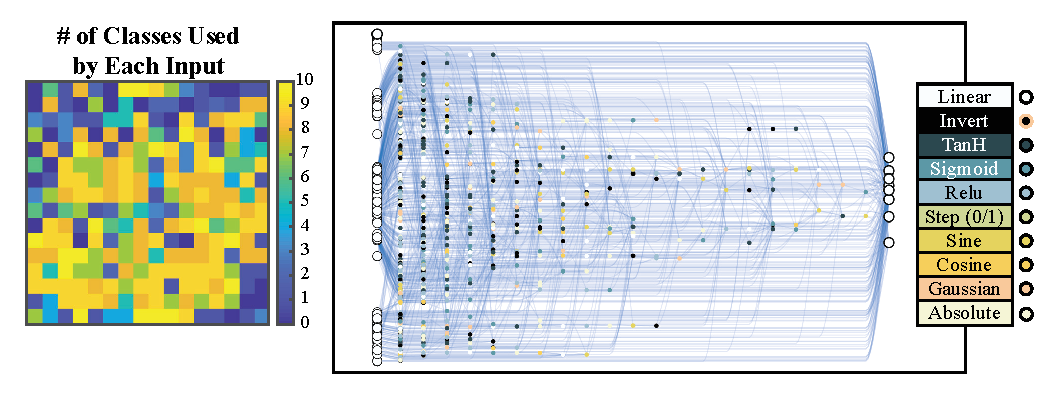
\includegraphics[width=1.0\textwidth]{img/champ_mnist_reduce_small.pdf}   
    %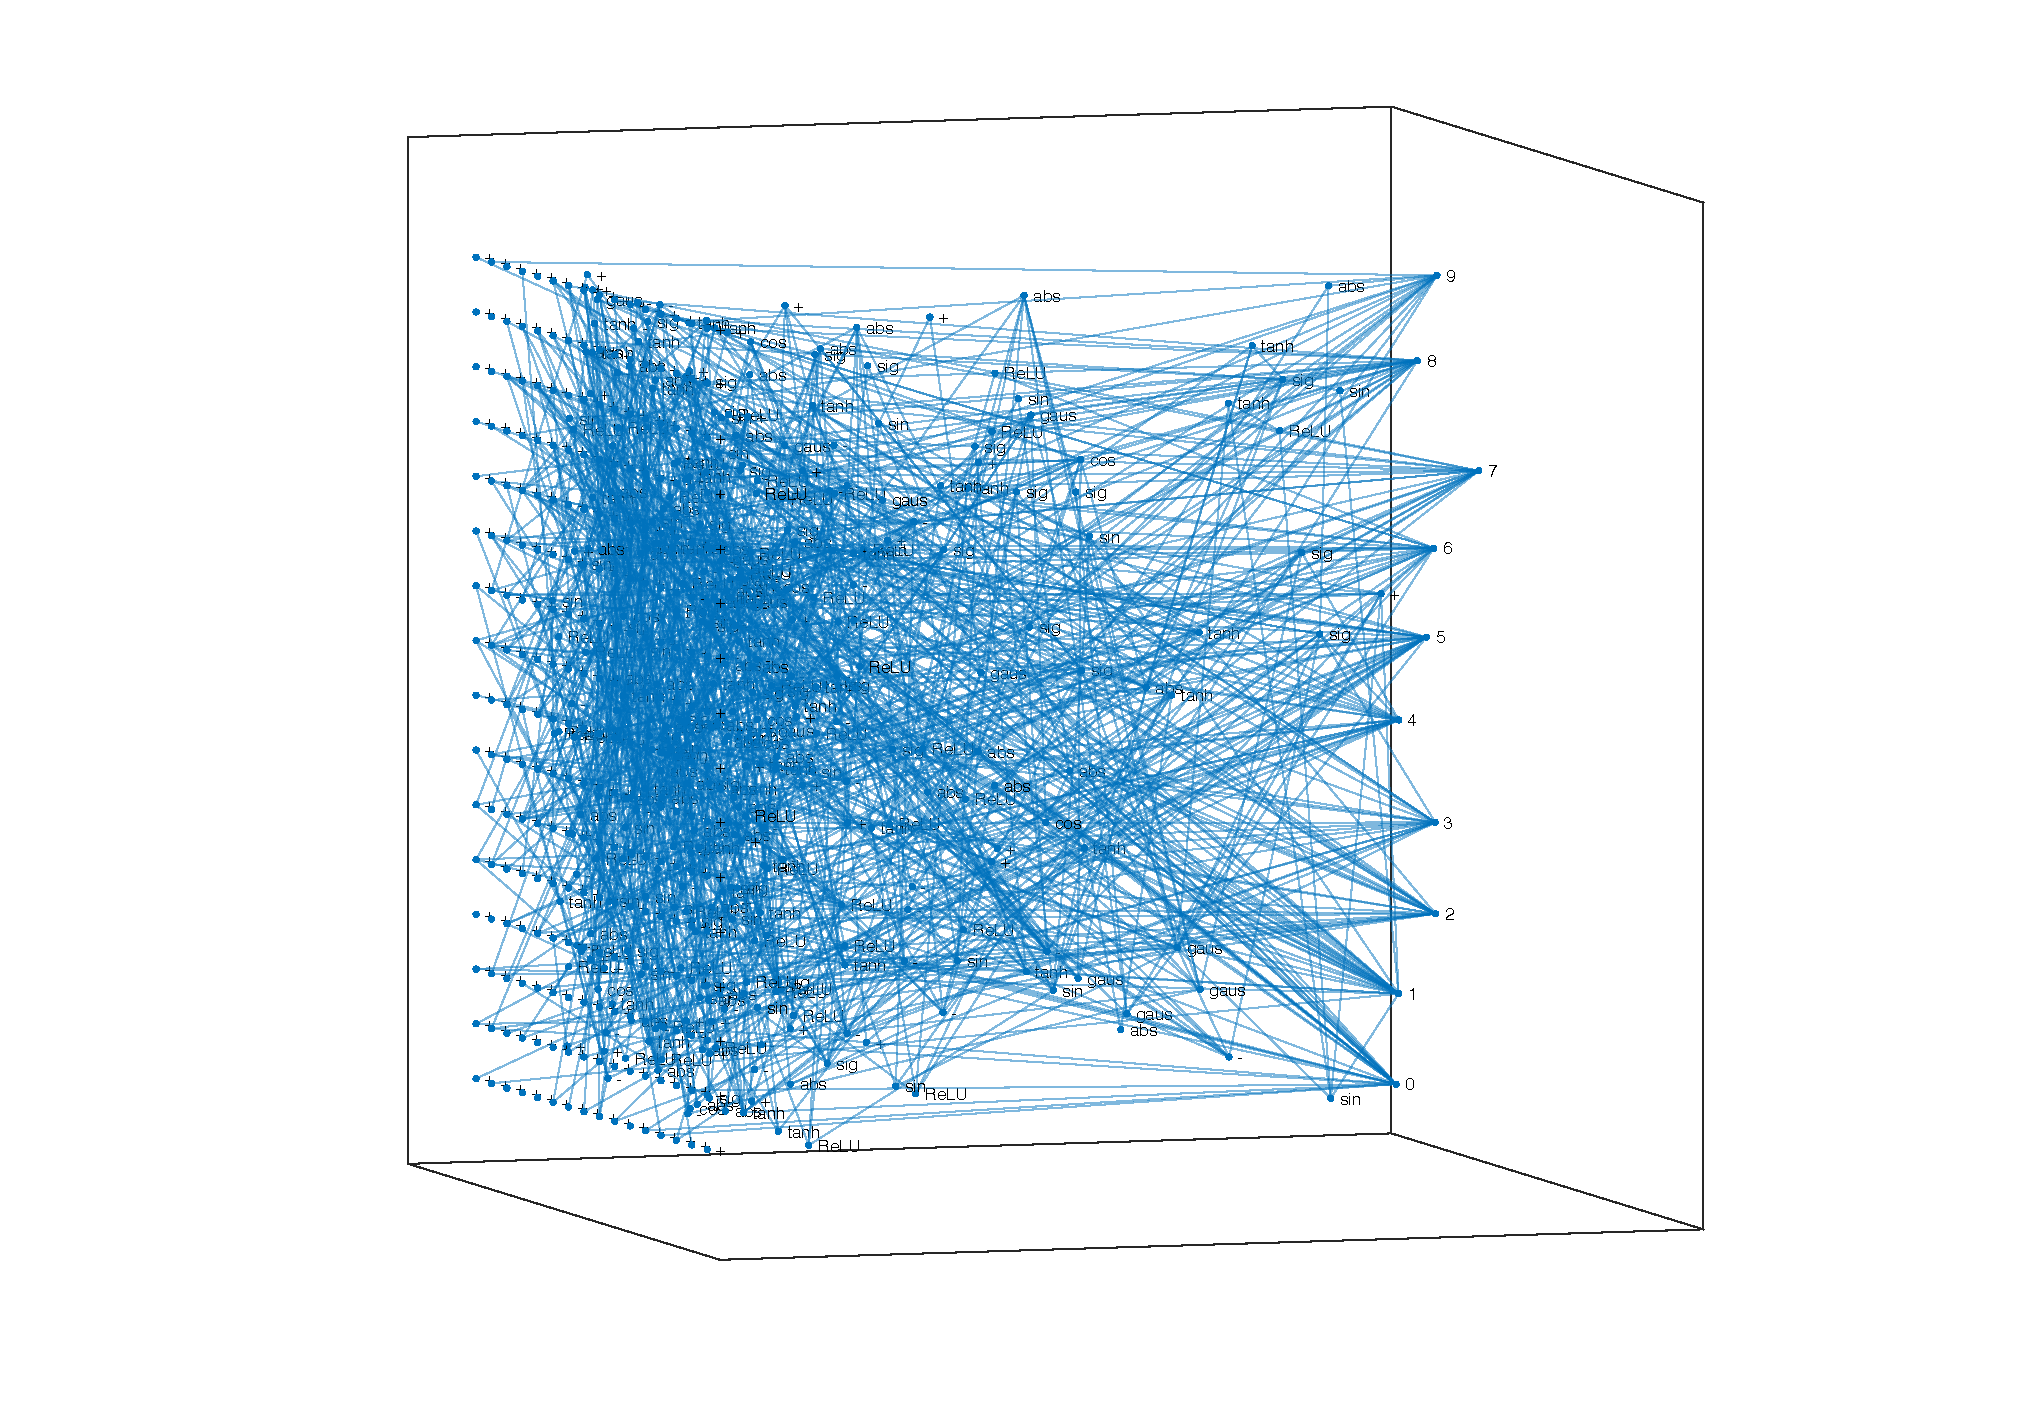
\includegraphics[width=0.45\textwidth]{supplemental/mnist_data/champ_mnist_net.pdf}   
    %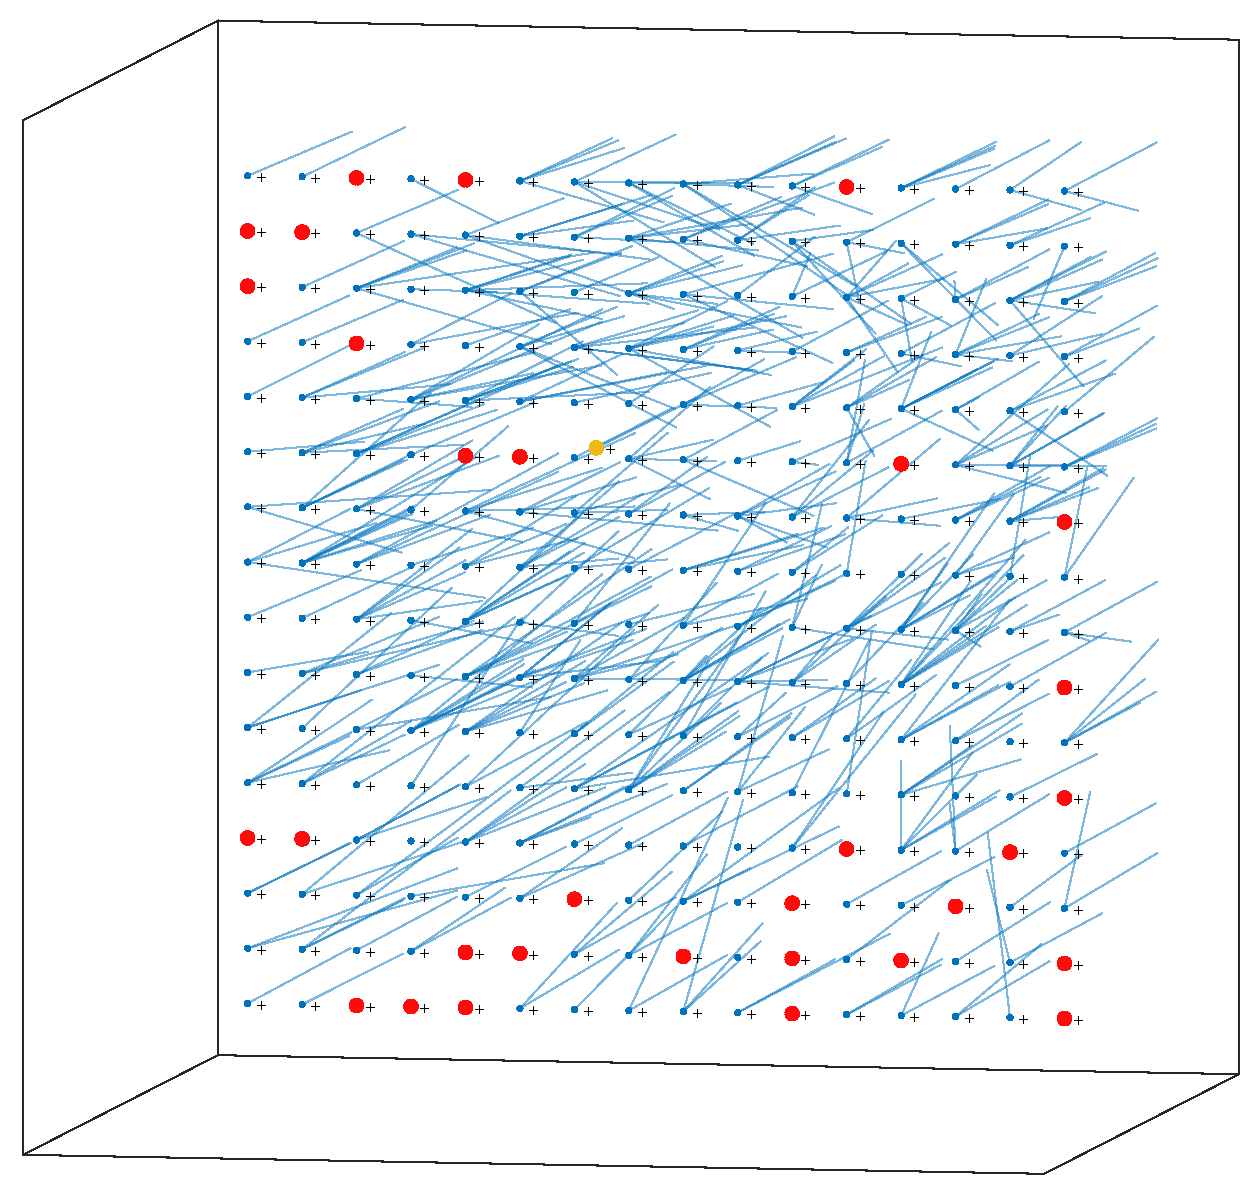
\includegraphics[width=0.45\textwidth]{supplemental/mnist_data/champ_mnist_net_input.pdf}  
\vskip -0.05in % useful knobs to optimize layout
    \caption      
    {     
	\textit{MNIST classifier network (1849 connections)}
	\newline
	Not all neurons and connections are used to predict each digit. Starting from the output connection for a particular digit, we can trace the sub-network and also identify which part of the input image is used for classifying each digit. Please refer to the \href{\websiteurl}{supplementary website} for more detailed visualizations. 
    }         
    \label{fig:mnistfull}
\vskip -0.15in % useful knobs to optimize layout
\end{figure}

